\section{Game Design Document}
\begin{figure}[ht]
\centering
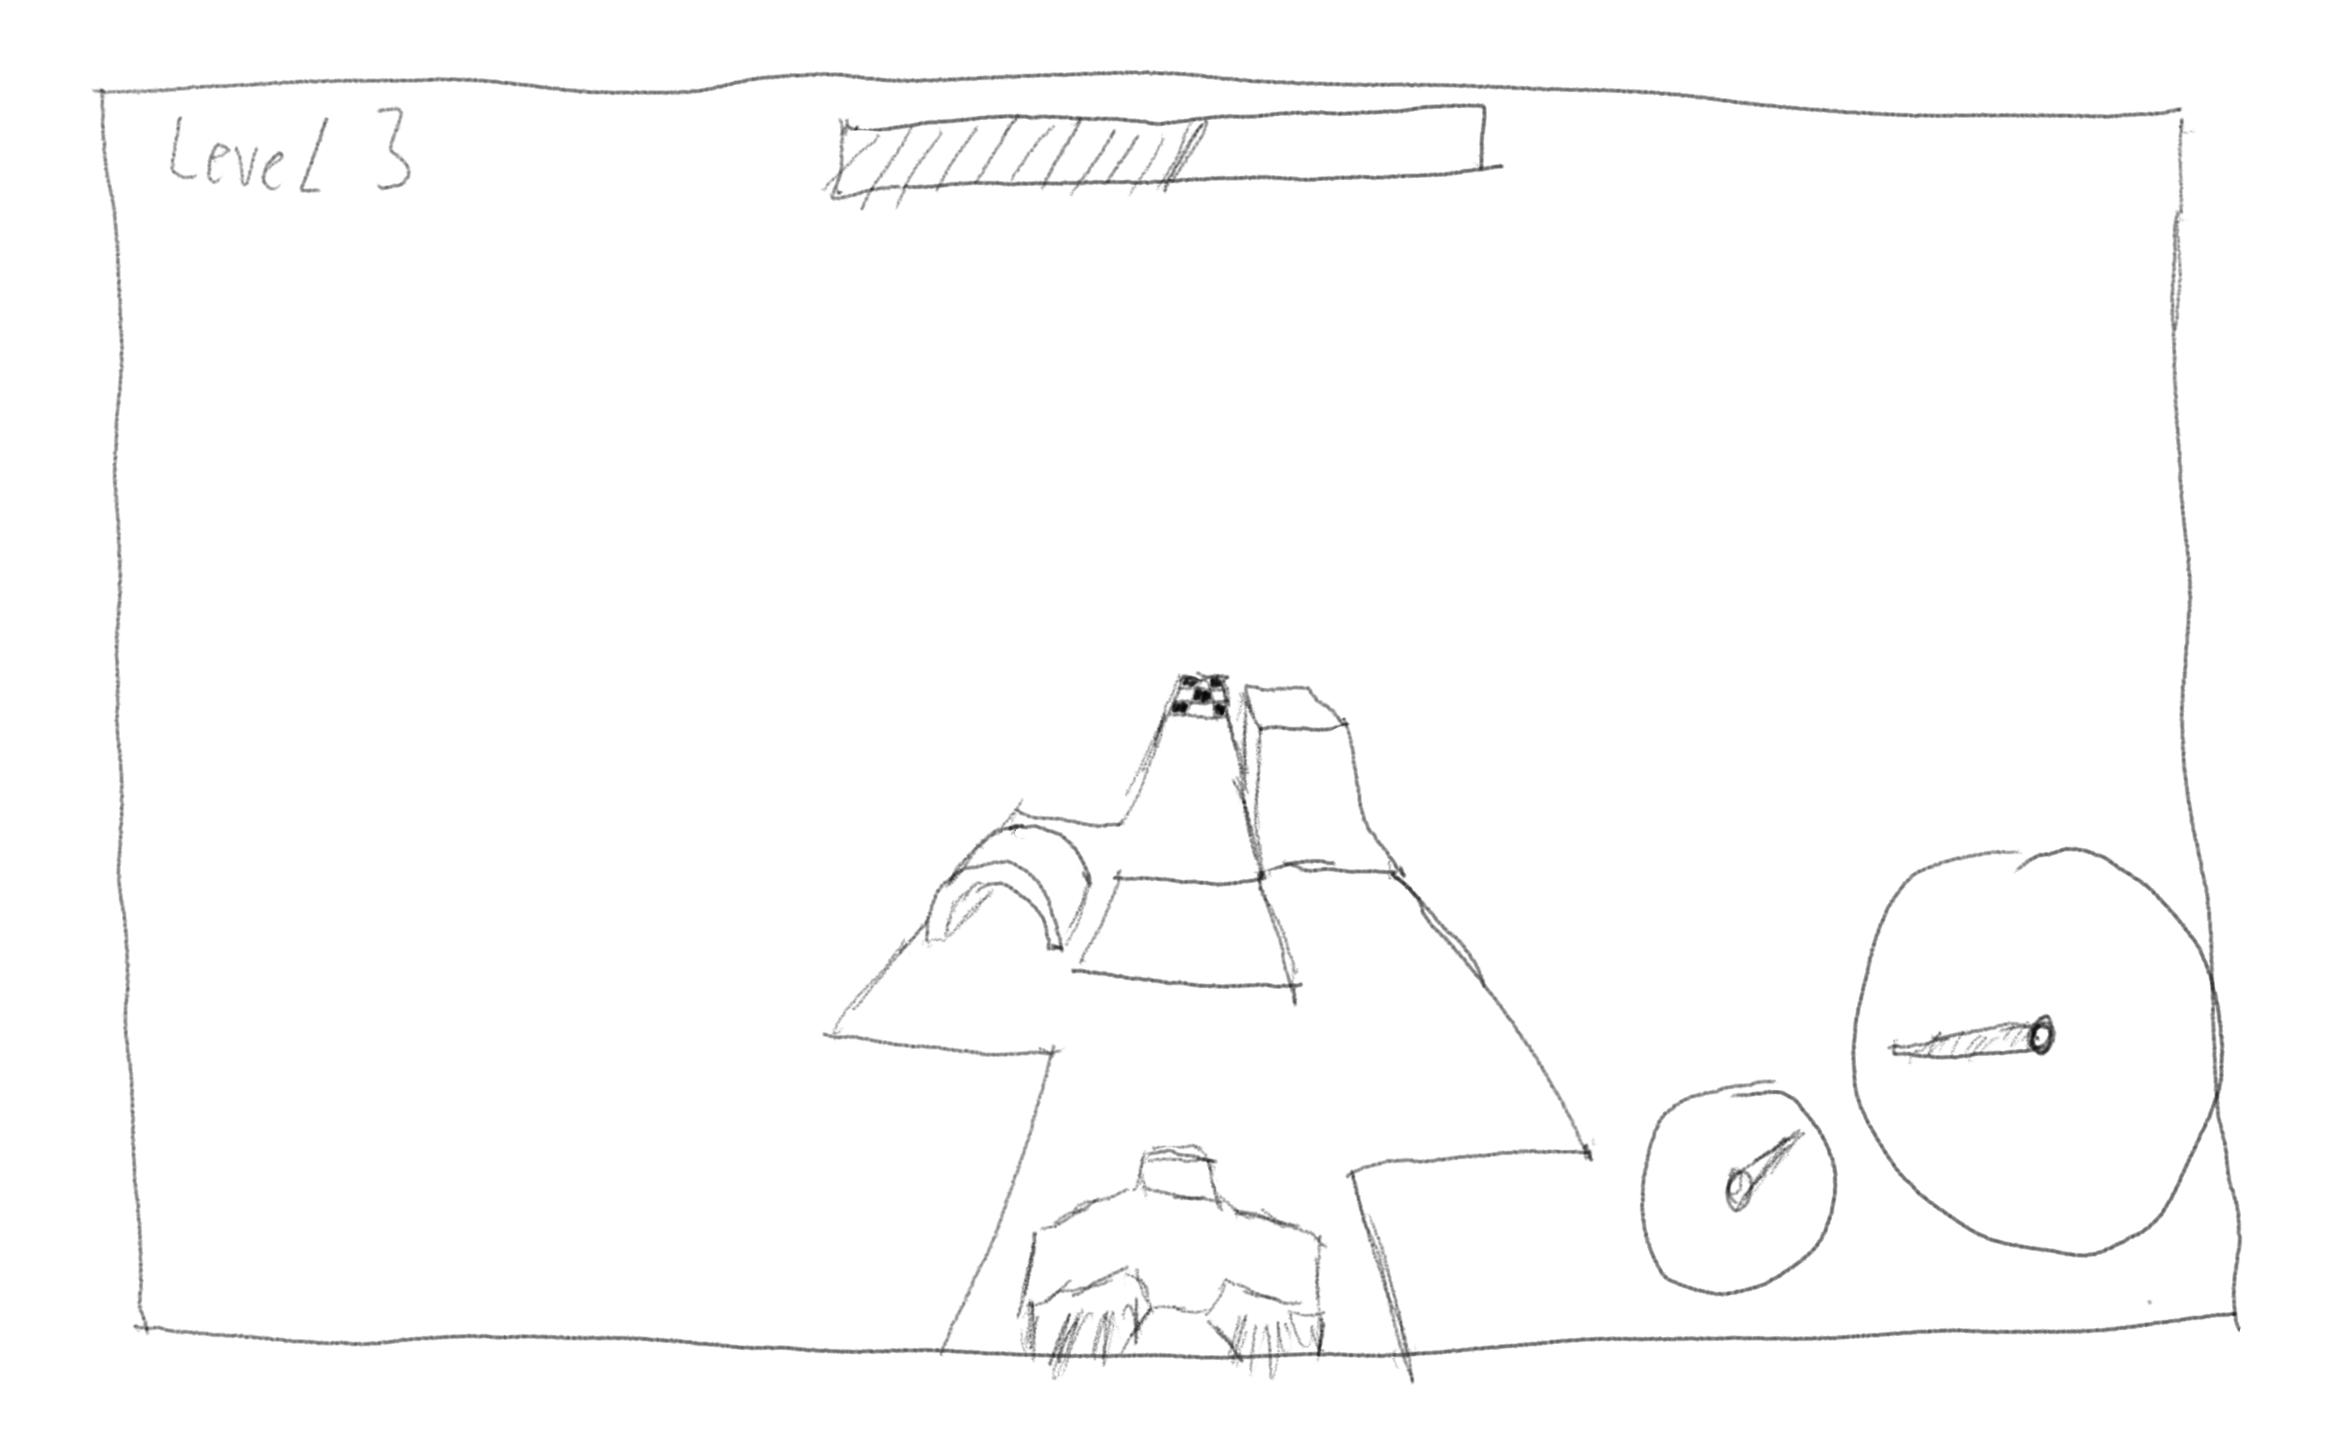
\includegraphics[width=.8\textwidth]{gfx/mockup.png}
\caption{Handskizze der Spielidee}
\end{figure}
\subsection{Spielobjekte}
Die Spielfigur ist ein Raumschiff, welches sich auf der Bahn bewegen kann. Auf der Bahn befinden sich Hindernisse in Form von Tunnel, Barrikaden und Abgründen. Außerhalb der Bahn befindet sich ebenfalls ein Abgrund.\\
Die Bahn kann auf zwei unterschiedlichen Ebenen verlaufen, wobei der Spieler entweder per Sprung oder Rampe die Ebene wechseln kann.

\subsection{User Interface}
Das User Interface zeigt eine Anzeige für die aktuelle Geschwindigkeit und den verbleibenden Kraftstoff in Form von Rundinstrumenten. Der Fortschritt im aktuellen Level wird als horizontaler Balken am oberen Bildschirmrand dargestellt, der sich mit zunehmender erfolgreich absolvierter Strecke füllt. Außerdem wird die Nummer des Levels, in dem sich der Nutzer aktuellen befindet, angezeigt.

\subsection{Sounds}
Bestimmte Spielsituationen, wie zum Beispiel das Beenden eines Levels, eine Kollision mit einem Hindernis und Springen, werden von entsprechenden und zum Thema des Spiels passenden Geräuscheffekten untermalt. Außerdem wird das Klicken eines Knopfes im Menü auch durch einen Ton an den Spieler rückgemeldet.

\subsection{Steuerung}
Das Spiel wird mit dem \textit{Smovetec} Fahrradergometer gesteuert. Durch die Trittfrequenz wird die Geschwindigkeit des Raumschiffs beeinflusst. Die Neigung des Ergometers hingegen lässt das Raumschiff nach Links oder Rechts lenken. Um mit dem Raumschiff springen zu können, muss der Spieler eine Taste am Griff des Ergometers betätigen. Eine weitere Taste lässt den Spieler das aktuelle Level unmittelbar neu starten.

\subsection{Levels}
Es gibt eine feste Anzahl von Levels. Mit dem Erreichen eines höheren Levels steigt auch der Schwierigkeitsgrad und neue Elemente werden schrittweise eingeführt. Die Level befinden sich in verschiedenen Umgebungen, was man anhand der veränderten Hintergründe und Texturen erkennt, sich aber nicht auf das Verhalten des Spiels auswirkt.